\documentclass[border=4pt]{standalone}
\usepackage[utf8]{inputenc}
\usepackage[T1]{fontenc}
\usepackage{lmodern}
\usepackage{amsmath,amssymb,mathtools}
\usepackage{tikz}
\usetikzlibrary{calc,decorations.pathreplacing,angles,quotes}
\usepackage{pgfplots}
\pgfplotsset{compat=1.18}
% Figura extraída de la Tarea 11 de Cálculo I (primer semestre).
\begin{document}
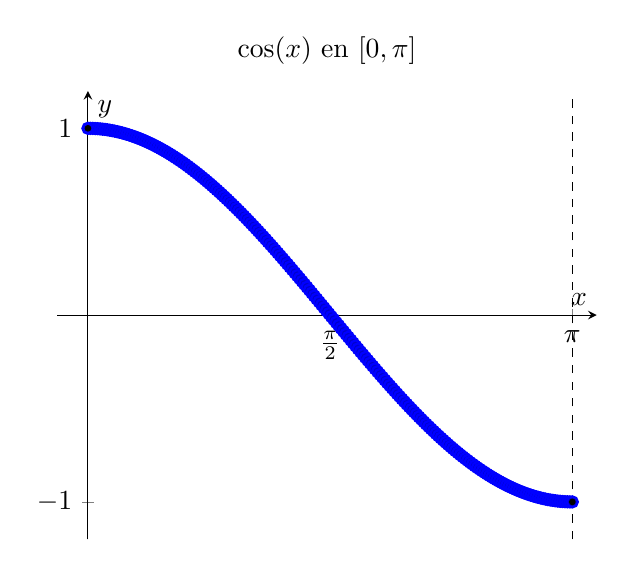
\begin{tikzpicture}
        \begin{axis}[
        domain=0:3.1416,samples=200,
        xmin=-0.2,xmax=3.3,ymin=-1.2,ymax=1.2,
        axis lines=middle,xlabel={$x$},ylabel={$y$},
        xtick={0,1.5708,3.1416},
        xticklabels={0,\(\tfrac{\pi}{2}\),\(\pi\)},
        ytick={-1,0,1},title={\(\cos(x)\) en \([0,\pi]\)}
        ]
        \addplot+[thick]{cos(deg(x))};
        \addplot[only marks,mark=*,mark size=1pt] coordinates {(0,1)(3.1416,-1)};
        \draw[dashed](axis cs:0,-1.2)--(axis cs:0,1.2);
        \draw[dashed](axis cs:3.1416,-1.2)--(axis cs:3.1416,1.2);
        \end{axis}
    \end{tikzpicture}
\end{document}
